\documentclass[sigconf,nonacm]{acmart}

% --- course paper: strip ACM boilerplate, keep the official sigconf 2-column look ---
\settopmatter{printacmref=false, printfolios=true}
\setcopyright{none}
\renewcommand\footnotetextcopyrightpermission[1]{}
\pagestyle{plain}

\usepackage{graphicx}
\usepackage{booktabs}

\begin{document}

\title{Draft Doesn't Decide It: Champion Picks are Near-Uninformative for
High-Elo League of Legends Win Prediction}
\subtitle{A clean negative result for the draft, and a region- and
patch-invariant signal from early objectives across NA, KR, and EUW}

\author{Yonghao Wang}
\affiliation{%
  \institution{DSC 148, University of California San Diego}
  \city{La Jolla}
  \state{CA}
  \country{USA}}
\email{yonghaowang16@gmail.com}

\begin{abstract}
We ask what actually predicts the winner of a \emph{high-elo} League of Legends
game. We collect \textbf{51,000} apex-ladder matches (50,999 labeled) from three
regions---NA, KR, EUW---via the Riot Match-V5 API (patches 16.9--16.11, Apr--May
2026), and predict whether the blue side wins. We compare two leakage-clean
feature regimes: \emph{draft-only} (champion picks, bans, summoner spells) and
\emph{draft + four first-objective} flags. \textbf{Finding 1 (negative):} at the
top of the ladder the draft is near-uninformative---every draft-only model sits
on the majority floor (AUC $\approx 0.54$), and once features are matched a
gradient-boosted model does not beat logistic regression
($\Delta\text{AUC} = -0.002$, $p = 0.67$). \textbf{Finding 2:} adding early
objectives recovers a strong signal (AUC $\approx 0.79$, first tower dominant)
that is remarkably stable across regions ($3\times3$ transfer gap 0.003) and
patches ($p = 0.89$ for a patch feature). High-elo red side wins 54.2\%, with KR
closest to even---a descriptive MMR-matching effect. We report $1000\times$
bootstrap confidence intervals throughout and a labeled leakage control (AUC
0.998). A live interactive demo is deployed at
\texttt{lol-win-predictor-web.onrender.com}.
\end{abstract}

\keywords{esports analytics; win prediction; negative result; cross-region
generalization; gradient boosting; SHAP; data leakage}

\maketitle

\section{Introduction}
The intuition behind League of Legends (LoL) win prediction is that the
\emph{draft}---which ten champions each team picks---should matter a great deal.
Champions have lopsided matchups, and ``draft diff'' is a staple of community
discourse. But is the draft actually informative once every player executes
competently? We study this at the very top of the ranked ladder
(Challenger/Grandmaster/Master), where mechanical execution is near-uniform and
any predictive content of the draft should be most isolated.

We ask three questions. (i) How much of the outcome can the pre-game draft alone
predict in high elo? (ii) How much does adding the earliest in-game objectives
(first blood, tower, dragon, rift herald) recover? (iii) Does whatever signal
exists generalize across regions and patches, or is it region-specific? To
answer them cleanly we enforce a strict leakage discipline, match feature sets
before comparing models, and attach $1000\times$ bootstrap confidence intervals
to every contrast so that tiny, sample-driven gaps are not mistaken for real
effects.

\noindent\textbf{Contributions.} (1) A \emph{clean negative result}: in high elo,
champion picks are near-uninformative---draft-only models do not measurably beat
the majority floor, and nonlinearity buys nothing once features are matched.
(2) A \emph{recovered, invariant signal}: early objectives lift AUC to
$\approx 0.79$ and that signal is nearly identical across three regions and three
patches---what is predictable is region-agnostic game mechanics, while region
differences live only in the (unpredictable) champion-preference meta. (3) A
\emph{descriptive} account of the high-elo red-side advantage and its regional
spread. (4) A rigorous methodology---bootstrap significance, a labeled leakage
control, feature-matched ablations---packaged with a deployed, interactive demo.

\section{Related Work}
\textbf{Composition-only models.} Predicting LoL outcomes from champion
composition \emph{alone} is weak: community ML projects report $\approx 55\%$
(Naive Bayes 55.3\%) and $\approx 53\%$ (tuned random forest) accuracy~\cite{comp}.
A standard explanation is self-optimization---because players draft to counter
and balance, the champion-vs-champion advantage is largely arbitraged away,
pushing a pure-composition predictor toward the 50\% coin-flip. Our high-elo
setting is the extreme of this mechanism.

\textbf{Adding player skill.} The signal lives in
\emph{player-on-champion mastery}, not the draft. Do et al.~\cite{do2021} reach
\textbf{75.1\%} accuracy at champion-select from players' experience on their
picked champions, concluding that individual champion skill matters
``regardless of team composition''; summing each player's per-champion win rate
has been reported as high as $\approx 93\%$~\cite{do2021}. Peer-reviewed work that
combines pre-game and in-game predictors improves further and notes early-game
events are \emph{less} predictive than late-game ones~\cite{combined}. The lever
we deliberately do not pull is player-on-champion mastery (not a direct Match-V5
endpoint); we return to it as the natural next step.

\textbf{Side and region.} A blue/red asymmetry is documented; community and
industry analyses report a larger red edge at the top of the ladder---red
$\approx 53\%$ vs blue $\approx 47\%$ in Master+~\cite{redside}. The proposed
mechanism is MMR matching: at the apex ladder few players queue at once, so the
two teams' MMR cannot always be balanced, and the side seeded with the
higher-MMR players (historically red) wins more often~\cite{redside}. This
predicts a region with a larger, more evenly-matched apex pool should sit closest
to 50/50---consistent with our KR observation (\S\ref{sec:data}). We treat all of
this as descriptive/correlational, not causal.

\textbf{Our position.} Relative to prior work we contribute a high-elo-specific
study across three regions, a rigorously-tested \emph{negative} result for the
draft (with confidence intervals rather than point estimates), an explicit
invariance test for the recovered objective signal, and a deployed demo for
inspection.

\section{Dataset and Exploratory Analysis}
\label{sec:data}
\textbf{Collection.} Seeded from each region's apex league lists
(Challenger--Master), we pull ranked matches through the Riot Match-V5 API with
correct regional routing (NA$\rightarrow$americas, KR$\rightarrow$asia,
EUW$\rightarrow$europe), parallelized across the three regional hosts and
deduplicated by \texttt{matchId}. The corpus is \textbf{51,000} matches---17,000
each from NA, KR, and EUW---on patches \textbf{16.9--16.11} (mostly 16.10), played
\textbf{2026-04-29} to \textbf{2026-05-30}. We drop one match with
\emph{winner}$=0$, leaving \textbf{50,999} labeled games. Every \texttt{matchId}
is round-tripped against the API and the final CSV contains \textbf{no player
identifiers} (no PUUIDs or summoner names).

\textbf{Leakage taxonomy.} We partition fields into \emph{safe} $=$ draft (picks,
bans, summoner spells); \emph{allowed} $=$ the four first-objective flags (blood,
tower, dragon, rift herald); and \emph{leaky} $=$ end-of-game state (kill counts,
first inhibitor, first baron, game duration). The leaky columns are permanently
excluded from all real results (\S\ref{sec:results} quantifies why).

\begin{figure}[t]
\centering
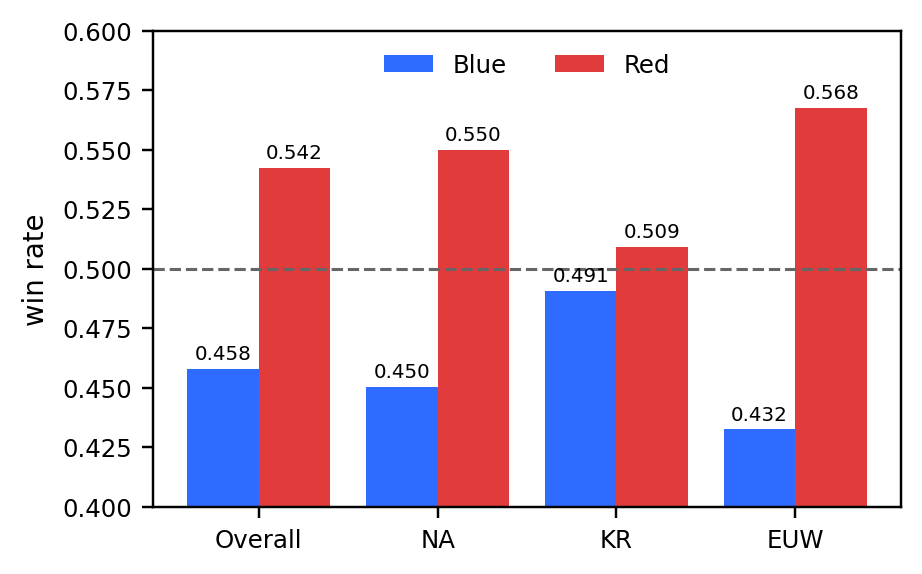
\includegraphics[width=\columnwidth]{fig1_side.png}
\caption{Win rate by side. High-elo red side wins \textbf{54.2\%} overall (blue
45.8\%). The bias is region-dependent---KR is closest to even (blue 49.1\%), EUW
most red-favored (blue 43.3\%)---consistent with an MMR-matching account.
\emph{Design impact:} the majority floor is 54.2\%, the bar every model must
clear, and side is a useful prior, motivating distinct blue/red feature blocks.}
\label{fig:side}
\end{figure}

\textbf{(1) Side and region.} Figure~\ref{fig:side} shows red wins 54.2\% overall
(blue 45.8\%), with a regional gradient: blue-win 49.1\% (KR), 45.0\% (NA), 43.3\%
(EUW). The ordering matches the apex MMR-matching account (\S2): KR's larger,
more evenly-matched apex queue sits closest to 50/50, while thinner NA/EUW queues
leave a bigger red edge. This sets the majority floor and motivates encoding side
explicitly.

\begin{figure}[t]
\centering
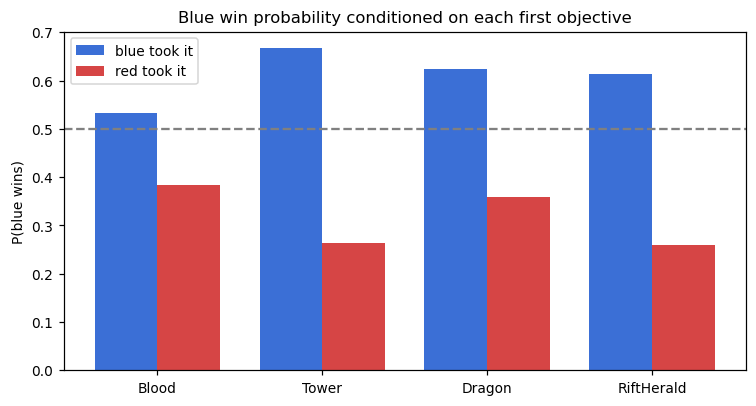
\includegraphics[width=\columnwidth]{fig2_objective.png}
\caption{Blue-win probability conditioned on which side took each first
objective. First tower is by far the strongest (gap \textbf{+0.405} between
blue-took and red-took), then rift herald (+0.354), dragon (+0.265), blood
(+0.148). \emph{Design impact:} directly motivates the draft+objectives regime.}
\label{fig:obj}
\end{figure}

\textbf{(2) Early objectives.} Conditioning blue's win probability on who took
each first objective (Fig.~\ref{fig:obj}) reveals a strong, monotone signal: the
blue-minus-red win gap is \textbf{+0.405} for first tower, +0.354 rift herald,
+0.265 dragon, +0.148 first blood. This is the lever the draft lacks, and
directly motivates regime B.

\begin{figure}[t]
\centering
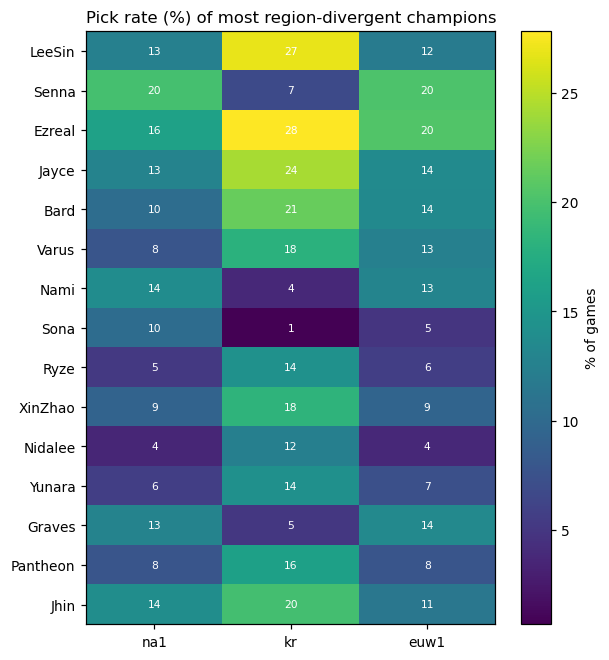
\includegraphics[width=\columnwidth]{fig3_region.png}
\caption{Pick rate (\%) of the most region-divergent champions. KR is distinct
(Lee Sin 27\% vs 12--13\%; Ezreal 28\%; enchanters avoided---Sona 1\%, Nami 4\%).
\emph{Design impact:} region lives in champion \emph{preferences}, which we show
are exactly the unpredictable part.}
\label{fig:region}
\end{figure}

\textbf{(3) Regional meta divergence.} Pick/ban rates differ sharply by region
(Fig.~\ref{fig:region}); KR favors Lee Sin and avoids enchanters relative to
NA/EUW. This frames our central story: regions differ in \emph{what they draft},
yet \S\ref{sec:results} shows the draft is the part that does not predict
outcomes.

\section{Predictive Task}
We predict a binary label: does blue (team 1 / teamId 100) win? We report
accuracy, blue-class F1, and ROC-AUC; AUC is our primary metric because it is
threshold- and prevalence-robust, which matters given the 54.2\% majority floor
that every model must beat. We define two feature \textbf{regimes}:
\textbf{A (draft-only)}---multi-hot champion picks, bans, and summoner spells;
and \textbf{B}---regime A plus the four symmetric first-objective flags. The
A$\rightarrow$B contrast is the paper's main experiment.

\textbf{Baselines.} Logistic regression and Bernoulli Naive Bayes. They are apt
foils for a composition signal: LR tests whether a \emph{linear} combination of
(binary) champion indicators separates wins, and NB tests a
conditional-independence view of champion presence---both natural null models for
``draft as a bag of champions.'' We hold the leaky columns out throughout, so no
model can see post-hoc game state.

\section{Model}
\textbf{Features.} Champions are encoded as a \emph{team-symmetric multi-hot} bag:
within a team, pick order is irrelevant, but blue and red occupy separate column
blocks so the model keeps a side prior. We never encode slot/lane positions---lane
is a UI convenience, not a model input---which prevents memorizing positions and
keeps the representation order-invariant. Region and patch enter as optional
one-hot features.

\textbf{Proposed models.} A \textbf{LightGBM} gradient-boosted ensemble
(optionally +region), and \textbf{ChampPoolNet}, a small network that learns a
32-d champion embedding and mean-pools it per team before a 64-unit head. The
embedding-vs-one-hot choice is set up as a feature-matched ablation: the same
head consumes either pooled embeddings or the raw multi-hot, isolating the
representation. ChampPoolNet is far more parameter-efficient ($\approx$149--157
input dims vs $\approx$709--717 for one-hot at equal AUC)---a promising
compactness we flag as potential, not a measured accuracy gain on 172 champions.

\textbf{Engineering.} Three real difficulties shaped the pipeline. (i) LightGBM
and PyTorch each bundle libomp; running them in one process \emph{deadlocks} via
duplicate OpenMP runtimes---fixed by single-threading and the duplicate-lib
guard. (ii) Sparse vectorization of the multi-hot bag was needed to keep
memory/time bounded. (iii) Under pandas 3.0 the new StringDtype turns empty cells
into real NaN, which silently corrupted encodings until coerced. (iv) For the
demo we found the all-objectives-\emph{none} state is \textbf{0.000\%} of training
data---out-of-distribution for regime B---so the pre-game screen serves the
genuinely-flat regime-A model and switches to B once any objective is set.

\textbf{Optimization.} LightGBM uses early stopping on a held-out split; a light
sweep settled on learning rate 0.03 and 31 leaves (\S\ref{sec:results} shows
insensitivity).

\textbf{Application.} We deploy the trained regime-B model behind a FastAPI
service and a Next.js front-end: a user enters two drafts and toggles early
objectives, and the blue win probability updates live with SHAP attributions. The
pre-game screen is near-flat as champions are swapped (the negative result, made
tangible); flipping \emph{first tower} makes the number jump---the paper's thesis
as an interaction.

\section{Results}
\label{sec:results}

\begin{table}[t]
\caption{Main results (all +region). Regime A (draft-only) vs B
(draft+objectives). Majority floor (predict red) $= 0.5422$ acc. In regime A every
AUC sits on the floor; in B all models reach $\approx$0.78--0.79. (OneHotMLP is
the one-hot control arm of the embedding ablation; its slightly higher B-F1 is
within noise and does not change the models' practical equivalence.) Numbers
copied from \texttt{ckpt4\_summary.txt}.}
\label{tab:main}
\footnotesize
\begin{tabular}{lccccc}
\toprule
Model & A acc & A AUC & B acc & B F1 & B AUC \\
\midrule
LogReg & 0.5423 & 0.5435 & 0.7215 & 0.6912 & 0.7846 \\
BernoulliNB & 0.5435 & 0.5448 & 0.7158 & 0.6940 & 0.7753 \\
LightGBM & 0.5504 & 0.5497 & 0.7232 & 0.6955 & \textbf{0.7914} \\
ChampPoolNet & 0.5429 & 0.5353 & 0.7236 & 0.6935 & 0.7884 \\
OneHotMLP & 0.5339 & 0.5439 & 0.7217 & 0.7058 & 0.7844 \\
\bottomrule
\end{tabular}
\end{table}

\textbf{Finding 1---the draft is near-uninformative (negative result).} In regime
A every model sits on the floor: AUC ranges 0.529--0.550 against a 0.5422 floor
(Table~\ref{tab:main}). Crucially, once features are matched the nonlinear model
does not help---LightGBM minus logistic regression is
$\Delta\text{AUC} = -0.0017$ ($p = 0.668$)---this feature-matched, no-region
contrast is the clean test of nonlinearity (the $+0.0063$, $p = 0.170$, with
region folds in the region term); learned embeddings minus one-hot is $-0.0086$
($p = 0.112$) (Table~\ref{tab:sig}). There is no detectable champion-interaction
signal in high elo. Measured as \emph{lift over the majority-class baseline}, the
gain is essentially nil---best regime-A accuracy is 0.5504 against the 0.5422
floor (under one point), and AUC 0.54--0.55 is barely above the 0.50 of random
ranking---even smaller than the $\approx$+5 points a (near-balanced) low-elo
composition-only model gains over its 50\% baseline~\cite{comp}:
self-optimization at its extreme.

\begin{table}[t]
\caption{$1000\times$ bootstrap paired AUC differences (* $=$ 95\% CI excludes 0).
In regime A only the (tiny) region term is significant; nonlinearity and
embeddings are within noise. In B the model gaps are significant but $<$0.02
AUC---statistically real, practically equivalent.}
\label{tab:sig}
\footnotesize
\begin{tabular}{lccc}
\toprule
Contrast ($\Delta$AUC) & $\Delta$ & 95\% CI & $p$ \\
\midrule
A: region alone (LGBM)       & $+$.0092 & [$+$.003,$+$.016] & .006* \\
A: nonlin$-$lin (LGBM$-$LR)  & $+$.0063 & [$-$.003,$+$.014] & .170 \\
A: embed$-$onehot            & $-$.0086 & [$-$.019,$+$.002] & .112 \\
B: LGBM$-$LR                 & $+$.0068 & [$+$.004,$+$.010] & .000* \\
B: LGBM$-$NB                 & $+$.0161 & [$+$.013,$+$.019] & .000* \\
B: embed$-$onehot            & $+$.0040 & [$+$.001,$+$.007] & .010* \\
B: +patch feature            & $+$.0001 & [$-$.001,$+$.001] & .892 \\
\bottomrule
\end{tabular}
\end{table}

\textbf{Finding 2---objectives recover a strong, invariant signal.} Regime B
reaches AUC $\approx 0.79$ (LightGBM 0.7914; accuracy 0.72), in line with the
$\approx$74\% accuracy reported for early-game / real-time models~\cite{combined}---first
tower dominates the SHAP attributions. We emphasize the honest reading of
Table~\ref{tab:sig}: in regime B LightGBM is \emph{statistically} the best
($p<0.001$ vs both baselines) but the margins are $<$0.02 AUC---the signal is in
the \emph{features, not the model}; the models are practically equivalent.

\textbf{Region.} Decomposed on AUC, region contributes a small but significant
+0.0092 in regime A ($p = 0.006$) and essentially nothing in regime B (it is
drowned out by the objectives). So the only predictive role of region is a weak
side-rate prior, not a draft effect.

\begin{table*}[t]
\caption{Cross-region $3\times3$ transfer (train-row $\times$ test-col, AUC).
Regime A is indistinguishable from chance everywhere (diag 0.527 / off-diag
0.512). Regime B transfers almost perfectly: diagonal 0.783 vs off-diagonal
0.779, gap only \textbf{0.003}. Numbers from \texttt{ckpt4\_summary.txt}.}
\label{tab:transfer}
\footnotesize
\begin{tabular}{lccc@{\hskip 3em}lccc}
\toprule
A (draft-only) & na1 & kr & euw1 & B (+objectives) & na1 & kr & euw1 \\
\midrule
train na1  & 0.522 & 0.499 & 0.531 & train na1  & 0.769 & 0.794 & 0.785 \\
train kr   & 0.512 & 0.535 & 0.521 & train kr   & 0.766 & 0.798 & 0.782 \\
train euw1 & 0.502 & 0.505 & 0.524 & train euw1 & 0.766 & 0.784 & 0.781 \\
\bottomrule
\end{tabular}
\end{table*}

\textbf{Cross-region transfer (Table~\ref{tab:transfer}).} Using the strongest
draft-only model, the A-matrix is flat at chance (mean diagonal 0.5271,
off-diagonal 0.5116; the +0.0156 gap is within noise). The B-matrix is the
headline invariance result: same-region 0.783 vs transfer 0.779, a 0.003
gap---the objective$\rightarrow$win relationship is essentially identical across
NA/KR/EUW. EUW-trained models lose accuracy on NA/KR (acc 0.658/0.641) while AUC
holds (0.766/0.784): a calibration/threshold drift, so a deployment should
re-calibrate its threshold per region rather than retrain.

\textbf{Patch robustness.} Per-patch AUC is 0.7888 / 0.7920 / 0.7963 for 16.9 /
16.10 / 16.11 (data is mostly 16.10); adding a patch one-hot moves AUC by +0.0001
($p = 0.892$)---no effect. \textbf{Hyper-parameters.} Regime-B AUC stays within
$\pm$0.01 across learning rate \{0.01--0.3\}, leaves \{15--127\}, and estimators
\{100--3000\}; the only thing that matters is using early stopping to avoid
over-fitting (AUC drops to 0.781 at 3000 fixed trees).

\textbf{Leakage control (not a real result).} Adding the banned end-of-game
columns to regime B inflates AUC from 0.7914 to \textbf{0.9983} (accuracy
0.721$\rightarrow$0.981)---a +0.207 AUC jump. We report this only to show how
post-hoc state would fabricate a near-perfect score, justifying the leakage
discipline.

\textbf{Case studies (regime B).} (i)~Most-confident-correct: NA1\_5557961866, red
took 3/4 objectives, P(blue)$=$0.056, red won. (ii)~A confident upset:
EUW1\_7870164239, red took 3/4, P(blue)$=$0.077, yet \emph{blue} won. (iii)~The
sharpest case---KR\_8201503869: red swept \textbf{4/4} objectives,
P(blue)$=$\textbf{0.098}, and blue still won. Together these show objectives are a
strong but non-deterministic signal: top-ladder comebacks are real, an
irreducible error floor that no pre/early feature set removes.

\section{Conclusion}
Three sentences summarize the study. In high elo the champion draft is
near-uninformative---a clean negative result, consistent with and at the extreme
of the $\approx$55\% reported for composition-only models at lower elos~\cite{comp}.
Early objectives recover a strong signal (AUC $\approx 0.79$) that is invariant
across three regions and three patches---what is predictable is region-agnostic
game mechanics, while region differences live only in unpredictable champion
preferences. The high-elo red-side advantage (54.2\%, KR closest to even) is a
descriptive MMR-matching pattern, not a causal claim.

\textbf{Limitations.} A single meta window (mostly patch 16.10) and, by design, no
player-on-champion mastery feature. \textbf{Future work.} The literature's missing
lever---Champion-Mastery and player-level history---is the natural next step; our
negative draft result makes that lever the precise thing to add to push pre-game
accuracy from $\sim$0.54 toward the $\sim$0.75 seen when player skill is
modeled~\cite{do2021}.

\section{Availability and Reproducibility}
\textbf{Live demo.} An interactive version is deployed at
\texttt{lol-win-predictor-web.onrender.com} (a static Next.js front-end over a
FastAPI service). Enter two drafts and toggle the early objectives: the blue win
probability and its top SHAP factors update live. In the all-objectives-none
state the number barely moves as champions are swapped---the negative result made
tangible (Fig.~\ref{fig:demo})---and flipping \emph{first tower} makes it jump
from $\approx$46\% to $\approx$77\%. (On the free tier the backend sleeps when
idle; the first load may take $\sim$30--60\,s while it wakes.)

\begin{figure}[t]
\centering
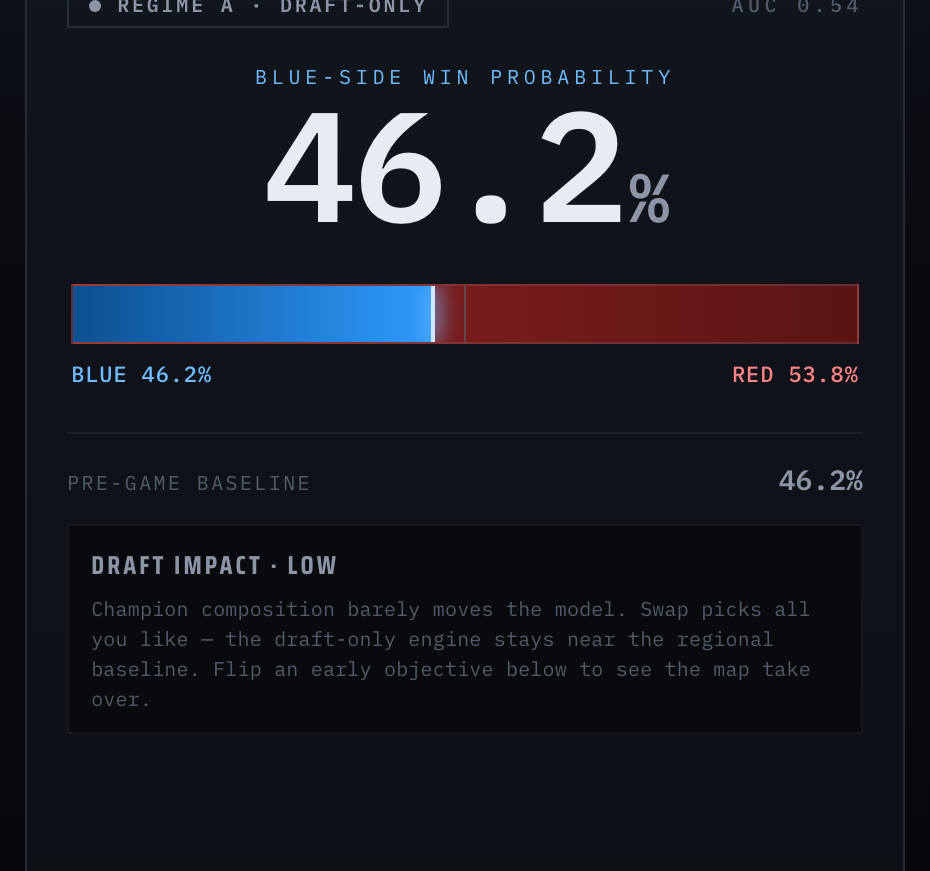
\includegraphics[width=0.9\columnwidth]{demo_wincore.png}
\caption{Center readout of the deployed demo in the all-objectives-none state:
regime A, \textbf{46.2\%} blue, ``DRAFT IMPACT $\cdot$ LOW---champion composition
barely moves the model.'' The negative result as a live readout; setting
\emph{first tower} switches to regime B and the number jumps to $\approx$77\%.}
\label{fig:demo}
\end{figure}

\textbf{Reproducibility.} All results use a fixed seed (42) and a single
stratified 80/20 split (50,999 $\rightarrow$ 40,799 train / 10,200 test), with the
champion vocabulary fit on the training split only; every contrast in
Table~\ref{tab:sig} is a $1000\times$ bootstrap. The exact figures in
Tables~\ref{tab:main}--\ref{tab:transfer} are emitted verbatim by the checkpoint
script (\texttt{ckpt4\_summary.txt}); the trained models and serving code
accompany this submission.

\begin{thebibliography}{9}
\bibitem{riot} Riot Games. \emph{Riot Developer Portal}---Match-V5 API and
regional routing (americas / asia / europe).
\texttt{developer.riotgames.com}.

\bibitem{comp} \emph{(community ML projects)} J.~Ou, \emph{Smart Winner Predictor
for League of Legends} (Weka, $\sim$50k Riot-API matches): Naive Bayes 55.3\% from
team composition; J.~Kang, \emph{lol-ai} (GitHub): tuned random forest
$\approx$53\%.

\bibitem{do2021} T.~D.~Do, S.~I.~Wang, D.~S.~Yu, M.~G.~McMillian, and
R.~P.~McMahan. \emph{Using Machine Learning to Predict Game Outcomes Based on
Player-Champion Experience in League of Legends.} Proc.\ 16th Int'l Conf.\ on the
Foundations of Digital Games (FDG~'21), 2021. 75.1\% at champion-select.
arXiv:2108.02799. \emph{Supporting:} T.~Huang, D.~Kim, V.~Leung (2015), summed
per-champion player win rates $\approx$92.8\% (Naive Bayes).

\bibitem{combined} \emph{Applications of Linear and Ensemble-Based Machine
Learning for Predicting Winning Teams in League of Legends.} Applied Sciences
15(10):5241, MDPI, 2025 (peer-reviewed): combining pre-game and in-game predictors
improves; early-game events are less predictive than late. \emph{Supporting:}
\emph{League of Legends: Real-Time Result Prediction}, arXiv:2309.02449, 2023
(LightGBM best, $\approx$74.4\% on early-game data).

\bibitem{redside} \emph{(community / industry analyses)} \emph{Red Side Advantage
in High-Elo League of Legends}, Riftfeed, 2024---per League of Graphs, Master+ red
$\approx$53\% vs blue $\approx$47\%, attributed to higher-MMR players placed on
red; A.~van Roon (Riot Games), official blue/red win rates by region, 2020 (via
Esports Tales).
\end{thebibliography}

\end{document}
